\documentclass[12pt]{article}

\usepackage[T2A]{fontenc}
\usepackage[utf8]{inputenc}
\usepackage[english, russian]{babel}

\usepackage[letterpaper,top=2cm,bottom=2cm,left=1.5cm,right=1.5cm,marginparwidth=1.75cm]{geometry}
\usepackage{float}
%\usepackage[bottom]{footmisc}

\usepackage{amsmath,amssymb}
\usepackage{graphicx}
\usepackage[colorlinks=true, allcolors=blue]{hyperref}
\usepackage{longtable,booktabs,array}
\usepackage{tablefootnote}
%\usepackage{footnote}
%\makesavenoteenv{longtable}
%\makesavenoteenv{tabular}
%\makesavenoteenv{table}
\usepackage{circuitikz}
\usetikzlibrary{fit}

\title{Лабораторная работа № 1 \\
``Фоторезистор как датчик освещённости. Датчик Холла для измерения магнитного поля'' \\
\large Сенсоры и сенсорные системы}

\begin{document}
\maketitle
\tableofcontents
\begin{abstract}
    Фоторезистор, датчик Холла. Устройство и прицип работы фоторезистора.
    Описание эффекта Холла. Принципиальные схемы включения датчиков.
\end{abstract}

\section{Теория}
\subsection{Фоторезисторы}

Изменение электрического сопротивления полупроводника, обусловленное непосредственным действием излучения, называют фоторезистивным эффектом, или внутренним фотоэлектрическим эффектом. Изменение сопротивления, или проводимости, вызывают изменением концентрации носителей заряда.

Фоторезисторы (рис.~\ref{phr}) предоставляют возможность определять интенсивность освещения. Они миниатюрны, недорогие, требуют мало энергии, легки в использовании, практически не подвержены износу. Именно из-за этого они часто используются в игрушках, гаджетах и приспособлениях. Фоторезисторы имеют различные размеры и технические характеристики, но в большинстве своем не очень точные. Каждый фоторезистор ведет себя несколько иначе по сравнению с другим, даже если они из одной партии от производителя. Различия в показаниях могут достигать 50\% и даже больше! Так что рассчитывать на прецизионные измерения не стоит. В основном их используют для определения общего уровня освещенности в конкретных, ``локальных'', а не ``абсолютных'' условиях.

\begin{figure}[H]
    \centering
    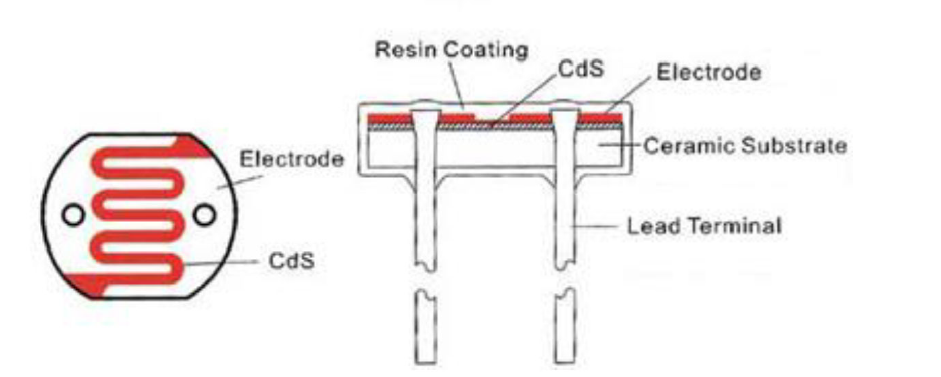
\includegraphics[scale=0.7]{images/photoresistor.png}
    \caption{Устройство фоторезистора}\label{phr}
\end{figure}

\textbf{Основные параметры фоторезисторов:}

\begin{itemize}
    \item
          диапазон сопротивления: от 200 кОм (темно) до 10 кОм (светло);
    \item
          диапазон чувствительности: чувствительные элементы фиксируют длины волн в диапазоне от 400 нм (фиолетовый) до 600 нм (оранжевый).
\end{itemize}

\subsubsection{Измерение уровня освещённости}

Как известно, сопротивление фоторезистора изменяется в зависимости от уровня освещения. Когда темно, сопротивление резистора увеличивается до 10 МОм. С увеличением уровня освещенности сопротивление падает. Приведенный ниже график (рис.~\ref{phrl}) приблизительно отображает зависимость сопротивление сенсора от уровня освещенности. В общем, характеристика каждого отдельного фоторезистора будет несколько отличаться, эти характеристики отображают только общую тенденцию.

\begin{figure}[H]
    \centering
    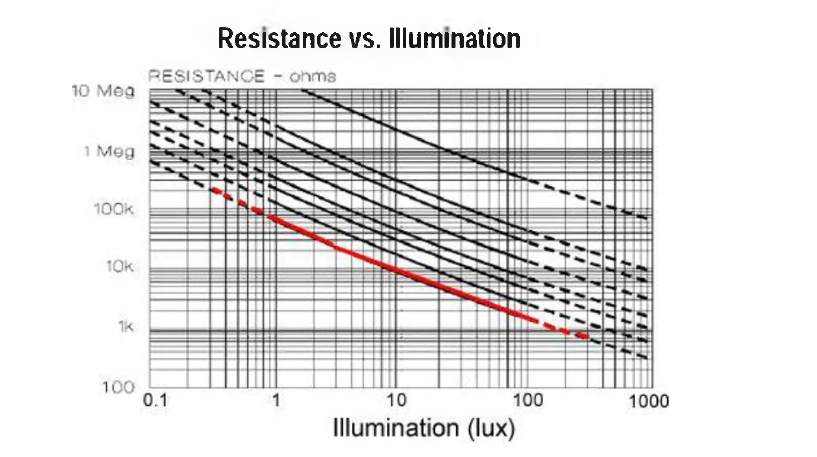
\includegraphics{images/illumination.png}
    \caption{Сопротивление фоторезистора в зависимости от уровня освещённости}\label{phrl}
\end{figure}

Обратите внимание, что характеристика нелинейная, а имеет логарифмический характер.

В качестве примера уровней освещенности при различных услолвиях ниже приведена таблица~\ref{illtable}.

\begin{table}[H]
    \caption{Уровни освещенности, воспринимаемые человеком}\label{illtable}
    \begin{longtable}[]{@{}l|l@{}}
        \toprule
        Освещение       & Пример                                                 \\
        \midrule
        \endhead
        0.002 лк        & Безлунное чистое небо                                  \\
        0.2 лк          & Необходимый минимум для экстренного освещения (AS2293) \\
        0.27-1 лк       & Чистое ночное небо при полной луне                     \\
        3.4 лк          & Граничный уровень освещённости под чистым небом        \\
        50 лк           & Жилая комната                                          \\
        80 лк           & Холл, туалет                                           \\
        100 лк          & Очень пасмурный день                                   \\
        300-500 лк      & Восход или закат в солнечный день. Хорошо освещеённый
        офис                                                                     \\
        1000 лк         & Вторая половина дня; освещение телевизионных студий    \\
        10000-25000 лк  & Полдень (не прямые солнечные лучи)                     \\
        32000-130000 лк & Прямые солнечные лучи                                  \\
        \bottomrule
    \end{longtable}
\end{table}

Фоторезисторы не воспринимают весь диапазон световых волн. В большинстве исполнений они чувствительны к световым волнам в диапазоне между 700 нм (красный) и 500 нм (зеленый) (см. рис.~\ref{phrspectr}).

\begin{figure}[H]
    \centering
    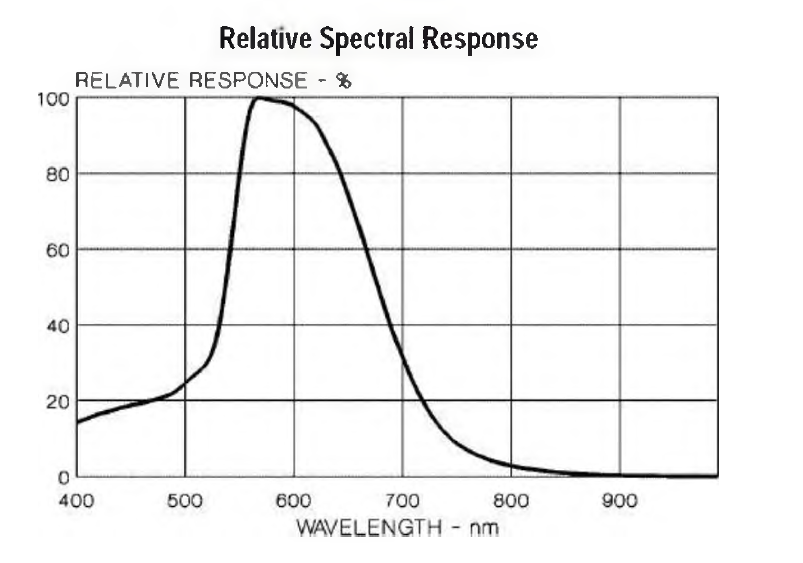
\includegraphics[scale=0.7]{images/photoresistor-wavelength.png}
    \caption{Спектральная чувствительность фоторезситора}\label{phrspectr}
\end{figure}

Фоторезистор включается в схему измерения, которая представляет собой делитель напряжения (рис.~\ref{phrcircuts}). Выходной сигнал снимается с нижнего плеча делителя, который представляет собой падение напряжения на фоторезисторе. Это напряжение можно измерить с помощью АЦП микроконтроллера.

\begin{figure}[H]
    \centering
    \begin{circuitikz}[european]
        \draw (0,0) node[ground](gnd){} to[phR, l=$R_{ph}$, name=photor, color=red] (0,3)
        to[R, l=$R$] (0,6) node[vcc](vcc){$V_{+}$};
        \draw (0,3) to [short, *-o] ++(3,0) node[above]{$V_{out}$};
        \node [anchor=north west] at ([xshift=5pt, yshift=-0pt]photor.south) {Фоторезистор};
    \end{circuitikz}
    \caption{Схема включения фоторезистора}\label{phrcircuts}
\end{figure}

Выходной сигнал схемы измерения - падение напряжения на фоторезисторе, вычисляется по следующей формуле:
\[
    V_{out} = V_{+} \cdot \frac{R_{ph}}{R + R_{ph}},
\]
где \(V_{+}\) - напряжение питания схемы (5В);

\(R_{ph}\) - сопротивление фоторезистора при данном уровне освещённости;

\(R\) - сопротивление верхнего плеча делителя напряжения, \(R=1 \ \text{кОм}\);

Отсюда по известному падению напряжения \(V_{+}\) и резистора \(R\) можно найти сопротивление фоторезистора:
\[
    R_{ph} = R \cdot \frac{V_{out}}{V_{+}-V_{out}}
\]

Связь сопротивления фоторезистора \(R_{ph}\) с уровнем освещенности \(L\) можно аппроксимировать следующей формулой:
\[
    L = 531.21 \cdot R_{ph}^{-5/4}
\]

\subsection{Датчик Холла}

Если через квадратную проводящую пластину пропустить постоянный ток, а саму пластину пронизать магнитным полем, чтобы линии индукции проходили через неё, то движущиеся по пластине электроны отклоняются силой Лоренца (рис.~\ref{halleff}). Таким образом, с одного края электронов будет больше, чем с другой. Возникает разность потенциалов, то есть напряжение. И чем больше ток и сильней поле, тем большая разность будет.

\begin{figure}[H]
    \centering
    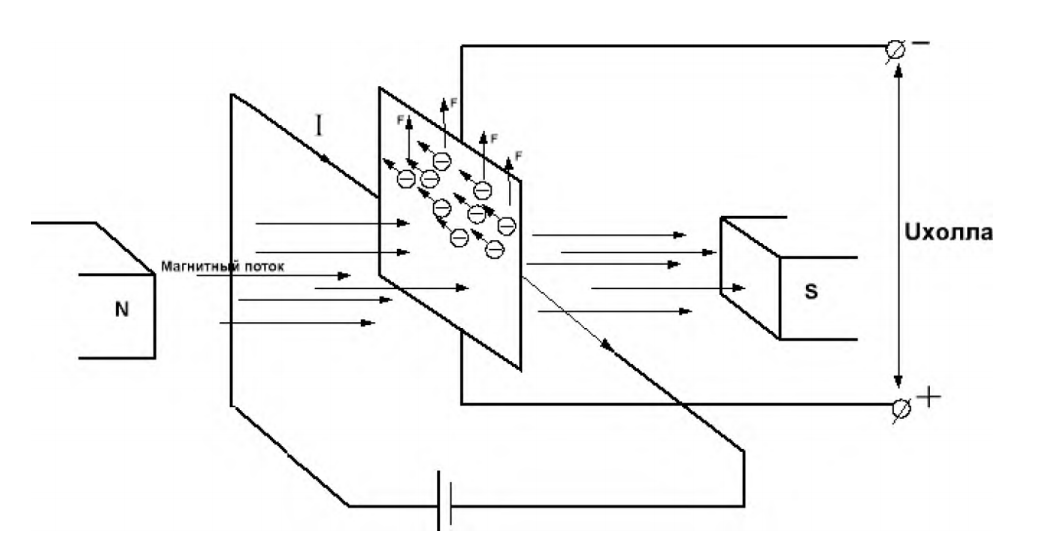
\includegraphics[scale=0.7]{images/hall-effect.png}
    \caption{Проявление эффекта Холла при протекании тока через тонкую
    пластину}\label{halleff}
\end{figure}

Разновидности датчиков на эффекте Холла:
\begin{itemize}
    \item
          \textbf{униполярные} (unipolar): низкое состояние выхода соответствует приложенному южному полюсу магнита, высокое - удалению магнита; на северный полюс датчики не реагируют;
    \item
          \textbf{биполярные} (bipolar): низкое состояние выхода соответствует приложенному южному полюсу магнита, высокое - северному полюсу; при удалении магнита состояние датчика не определено;
    \item
          \textbf{омниполярные} (latching): низкое состояние выхода соответствует приложенному южному полюсу магнита, высокое - северному полюсу; при удалении магнита состояние выхода не меняется, т.е. срабатывание датчика происходит только при смене полюсов.
\end{itemize}

В обучающем стенде представлен дискретный датчик магнитного поля на эффекте Холла. Сигнальный выход представляет из себя открытый коллектор, подтянутый резистором к питанию датчика (рис.~\ref{hallcircuts}).

\begin{figure}[H]
    \centering
    \begin{circuitikz}[european]
        \ctikzset{multipoles/dipchip/width=1}
        \draw (0,0) node[dipchip,
            num pins=6, hide numbers, no topmark,
            external pins width=0](hall){\large{X}};
        \draw (hall.n) -- ++(0,1) coordinate(pvcc0) -- ++(0,1) coordinate(pvcc) -- ++(0,1) node[vcc]{$V_{+}$};
        \draw (hall.s) -- ++(0,-2) coordinate(pgnd) -- ++(0,-1) node[ground]{};
        \draw (hall.bpin 5) -- ++(2,0) node[op amp, noinv input down, anchor=-](OA){};
        \draw (hall.bpin 2) -- ++(-1,0) coordinate(hallminus);
        \draw(OA.+) to [short, -] (OA.+ -| hallminus) -- (hallminus);
        \draw (OA.out) -- ++(1,0) node[schmitt,  anchor=in](sch_tr){}
        (sch_tr.out) to[R] ++(3,0) node[npn, anchor=B](Q){}
        (pgnd) to[short, *-] (pgnd -| Q.E) -- (Q.E)
        (Q.C) -- ++(0,0.5) -- ++(0.2,0) coordinate(outres0) -- ++(0.8,0) coordinate(outres) to[R=$R$] ++(0,2)
        coordinate(r_to_vcc);
        \draw (pvcc) to[short, *-] (pvcc -| r_to_vcc) -- (r_to_vcc);
        \draw (outres) to[short, *-o] ++(2,0) node[above]{$V_{out}$};
        \node [anchor=north west] at ([xshift=5pt, yshift=20pt]hall.north) {\text{Ч. э. на эффекте Холла}};
        \node [rectangle, draw, dashed, fit={(hall) (pvcc0) ([shift={(0mm,-5mm)}]pgnd) (outres0)}, label=above right:Датчик Холла](body){};
    \end{circuitikz}
    \caption{Внутренне устройство датчика Холаа и схема включения}\label{hallcircuts}
\end{figure}

Внутри микросхемы датчика сигнал с чувствительного элемента на эффекте Холла (генератор Холла) усиливается, далее через триггер Шмитта поступает на базу выходного транзистора, коллектор которого остается открытым. Схема подключения датчика включает в себя питание и подтягивающий резистор \(R\) на выход микросхемы датчика.

При поднесении к нему магнита нужной полярностью (правильной стороной) сигнальный вывод соединяется с общим проводом через n-p-n переход. Такие датчики как АЗ144 находят применение вместо морально устаревших герконов, в енкодерах, при измерении силы тока и в индикаторах вращения. Их можно применять как в релейной логике, просто подключив к выходу катушку электромагнитного реле, так и совместно с микроконтроллерами в качестве дискретного датчика холла.

\section{Лабораторная работа}

\subsection{Цель работы}

Знакомство со стендом: подключить модуль датчиков к модуля с микроконтроллером. Изучить основы работы с микроконтроллером, понятие простейшей периферии - порта и методики взаимодействия с ним. Изучить одну из разновидностей средств измерений - датчик. Овладеть знаниями о классификации датчиков. Определить, к какой группе датчиков следует относить датчик Холла и фоторезистор. Научиться получать правильные электрические показания с датчиков и преобразовывать в удобную для представления человека форму

\subsection{Оборудование}

Модуль датчиков. Модуль «Микроконтроллер ATMEGA32, компьютер/ноутбук.

\subsection{Ход работы}

\subsubsection{Подключение}

Подключите модуль "Микроконтроллер ATMEGA32", модуль "Модуль датчиков" к внешнему блоку питания (или у портам USB компьютера/ноутбука) с помощью кабеля USB. Выполните коммутацию модулей приборными проводами в соответствии с таблицей~\ref{labtable}  и с рис.~\ref{labscheme}.

\begin{figure}[H]
    \centering
    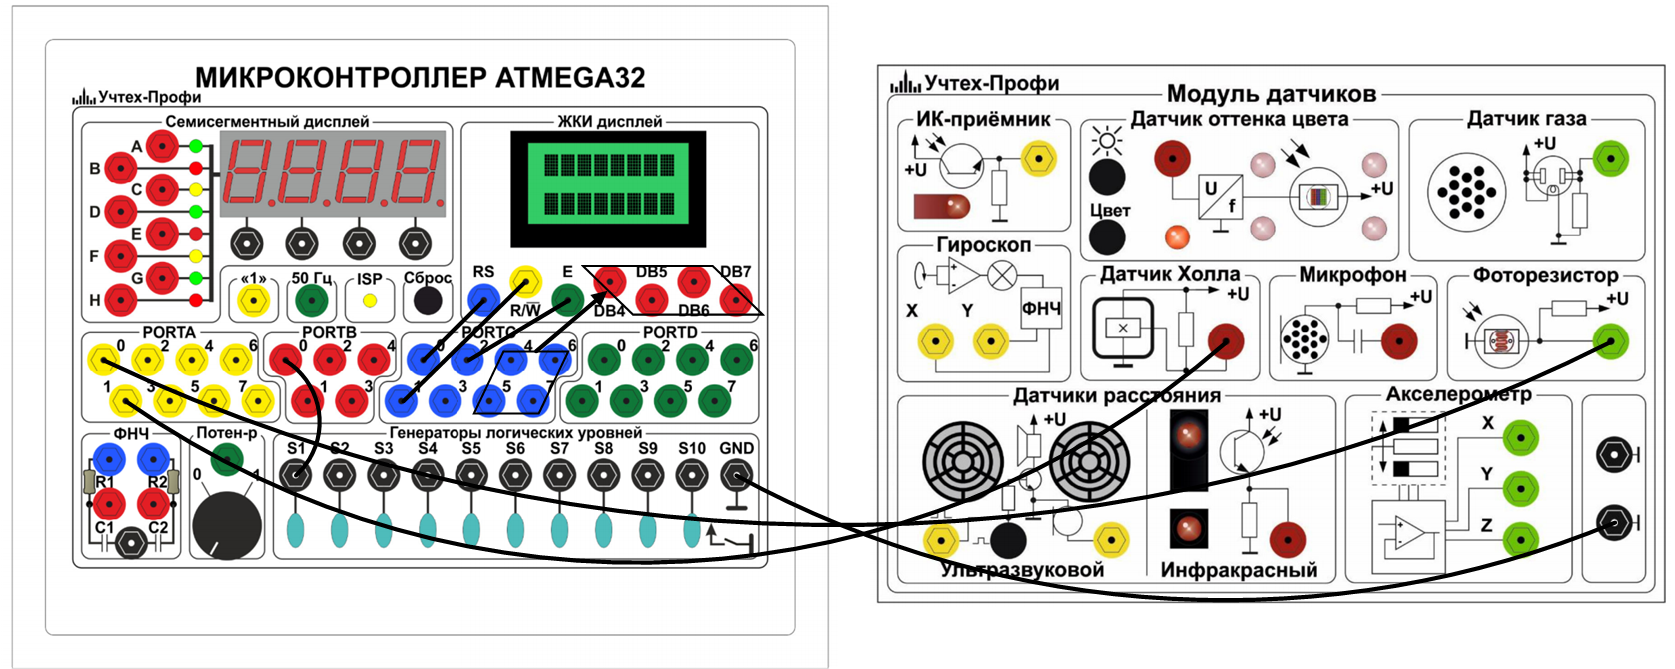
\includegraphics[scale=0.65]{images/lab1-scheme.png}
    \caption{Схема подключения модулей}\label{labscheme}
\end{figure}

\begin{table}[H]
    \caption{Коммутация модулей}\label{labtable}
    \begin{longtable}[]{@{}l|l@{}}
        \toprule
        Порт микроконтроллера ATMEGA32 & Назначение \\
        \midrule
        \endhead
        PORTD:0 & ЖК-дисплей: RS \\
        PORTD:1 & ЖК-дисплей: R/W \\
        PORTD:2 & ЖК-дисплей: E \\
        PORTD:4-7 & ЖК-дисплей: DB4-DB7 \\
        PORTA:0 & Фоторезистор \\
        PORTA:1 & Датчик Холла \\
        PORTB:0 & Генератор логических уровней: S1 \\
        \bottomrule
    \end{longtable}  
\end{table}

\subsubsection{Использование кода}

Для проведения измерений в лабораторной работе необходимо загрузить программу в микроконтроллер ATMEGA32. В папке \texttt{/src} лежат файлы исходного кода программы. Заголовочные файлы подключаемых модулей находятся \texttt{/include}. Основной выполняемый код находится в файле \texttt{/src/main.cpp}. Откройте его и проанализируйте код, который в нём содержится.

Запустите компиляцию и сборку прошивки нажав на кнопку "Build" на нижней панели VSCode. Затем загрузите файл прошивки в память микроконтроллера нажав на кнопку "Upload". После этого на ЖК-дисплее отобразятся измеряемые величины с подключённых датчиков. В случае с фоторезситором, на ЖК-дисплее будет отображно две строчки: сверху значение оцифрованное значение сигнала с фоторезистора 0-1023 ед., на нижней строчке будет отображено приблизительный уровень освещённости \(L\), в \([\text{лк}]\).

\subsubsection{Работа с фоторезистором}

\begin{enumerate}
    \def\labelenumi{\arabic{enumi}.}
    \item
      Переключите тумблер S1 генератора логических уровней в начальное
      положение. Тумблером S1 выбирается датчик, фоторезистор или датчик
      Холла, с которого в данный момент снимаются измерения.
    \item
      Используйте точечный источник света (например, светодиод телефона).
      Облучайте им фоторезистор и снимите несколько показаний оцифрованного
      напряжения с фоторезситора и уровня освещенности при различных
      расстояниях между источником света и фоторезистором. Используйте для
      этого линейку. Полученные значения для нескольких расстояний занесите
      в таблицу ниже. Проведите 5-10 измерений с различными расстояниями.

      \begin{table}[H]
        \centering
        \caption{Результаты измерений}\label{labtable0}
        \begin{tabular}{p{3cm}|p{3cm}|p{3cm}|p{3cm}|p{3cm}}
            \toprule
            Расстояние\linebreak \(H\), \(\text{мм}\) & Значение АЦП & 
            Напряжение \(V_{out}\)\tablefootnote{Разрядность АЦП микроконтроллера 10 бит, следовательно, диапазон значений АЦП 0..1023, где 1023 соответствует напряжению питания 5В.} & Сопротивление \(R_{ph}\), \(\text{кОм}\) & Уровень освещенности \(L\), \(\text{лк}\) \\
            \midrule
            5-10 измерений & - & - & - & - \\
            \hline
            - & - & - & - & - \\
            \hline
            - & - & - & - & - \\
            \bottomrule
        \end{tabular} 
    \end{table}
    \item 
      По полученным данным постройте график зависимости \(L=f(H)\) уровня освещенности \(L\) от расстояния до источника света \(H\). 

\end{enumerate}

\subsubsection{Работа с датчиком Холла}

\begin{enumerate}
    \def\labelenumi{\arabic{enumi}.}
    \item
      Переключите тумблер S1 генератора логических уровней в крайнее положение. Таким образом выбираем датчик Холла в качестве источника измерений микроконтроллера.
    \item
      Используя постоянный магнит проведите ряд измерения, поднося магниты обоими полюсами к датчика и фиксируя его показания. Определите максимальное расстояние, на котором датчик Холла срабаатывает на постоянный магнит. Сделайте вывод о типе датчика по его реакции на полюса магнита (униполярный, биполярный, оминполярный).
\end{enumerate}

\subsection{Вопросы}

\begin{enumerate}
    \def\labelenumi{\arabic{enumi}.}
    \item
      Дайте определение фоторезистивному эффекту. Устройство и принцип работы фоторезистора.
    \item
      Общая схема включения фоторезистора в измерительные схемы. Диапазон сопротивлений фоторезистора.
    \item
      В чем заключается эффект Холла? Какие существуют типы датчиков на эффекте Холла?
    \item
      Внутреннее устройство датчика Холла и схема его включения в измерительные схемы.
\end{enumerate}

\end{document}